\chapter{Graphical User Interface}
\label{user-gui}

Running \textttuse{frama-c-gui} or \textttuse{frama-c-gui.byte} displays the
\FramaC Graphical User Interface (GUI).

\section{\FramaC Main Window}

Upon launching \FramaC in graphical mode on some \C files, the following main
window is displayed (figure~\ref{fig:gui-init}):
\begin{figure}[htbp]
\begin{center}
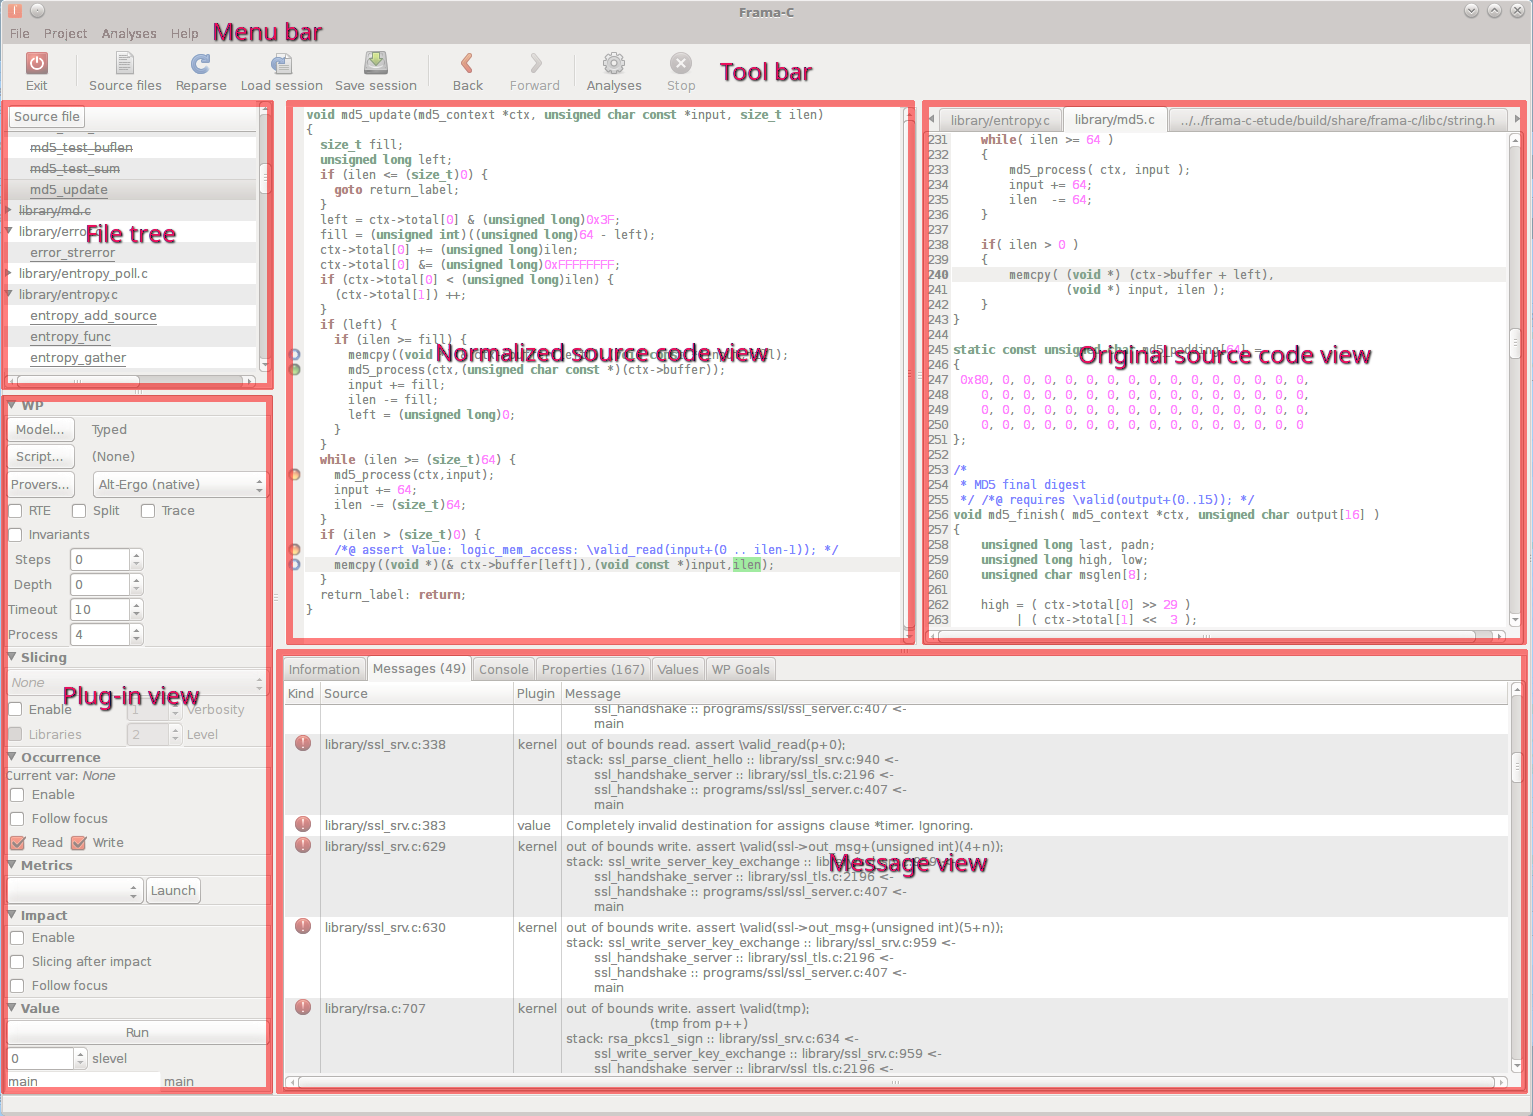
\includegraphics[width=0.95\textwidth]{gui-main-window.png}
\end{center}
\caption{Initial View}
\label{fig:gui-init}
\end{figure}

From top to bottom, the window is made of several separate sub-parts.

\begin{description}
\item [The menu bar] organizes the highest-level functions of the tool into
  structured categories. Plug-ins may also add their own entries in the
  ``Analyses'' menu.

\item [The toolbar] gives access to the main functions of the tool. They
  are usually present in one menu of the menu bar. Plug-ins may also add their
  own entries here.

\item [The file tree] provides a tree-like structure of the source
  files involved in the current analysis. This tree lists all the global
  variables and functions each file contains. Within a file, entries
  are sorted alphabetically, without taking capitalization into
  account. Functions are underlined, to separate them from variables.
  Plug-ins may also display specific information for each file and/or
  function. Finally, the ``Source file'' button offers some options to
  filter the elements of the file tree:
  \begin{itemize}
  \item The ``Hide variables'' and ``Hide functions'' options offer
    the possibility to hide the non-desired entries from the tree.

  \item The ``Flat mode'' option flattens the tree, by removing the
    filename level. Instead, functions and globals are displayed together,
    as if they were in a big namespace. This makes it easier
    to find a function whose only the name is known.

  \end{itemize}

\item [The normalized and original source code views] display the source code
  of the current selected element of the file tree and its normalized code (see
  Section~\ref{sec:normalize}). Left-clicking on an object (statement,
  left-value, \etc) in the normalized source code view displays information
  about it in the ``Information'' page of the Messages View and displays the
  corresponding object of the original source view, while right-clicking on
  them opens a contextual menu. Items of this menu depend on the kind of the
  selected object and on plug-in availability.

  \begin{important}
    Only the normalized source view is interactive: the original one is not.
  \end{important}

\item [The plug-ins view] shows specific plug-in interfaces. The interface
  of each plug-in can be collapsed.

\item [The messages view] contains by default six different pages, namely:

\begin {description}
\item [Information:] provides brief details on the currently
  selected object, or informative messages from the plugins.

\item [Messages:] shows important messages generated by the \FramaC kernel
  and plug-ins, in particular all alarms. Please refer to the
  specific documentation of each plug-in in order to get the exact form of
  alarms. Alarms that have a location in the original source can be
  double-clicked; this location will then be shown in the original and
  normalized source code viewers.\footnote{Notice however that the location
  in the normalized source may not perfectly correspond, as more
  than one normalized statement can correspond to a source location.}

\item [Console:] displays messages to users in a textual way. This
  is the very same output than the one shown in batch mode.

\item [Properties:] displays the local and consolidated statuses of
  properties.

\item [Values:] displays information relative to the Value Analysis
  plug-in.

\item [WP Goals:] displays information relative to the WP plug-in.

\end {description}

\end {description}

%% Displaying the GUI when running \FramaC may take a significant time. In such a
%% case, \FramaC does not display immediately the above mentioned main window but
%% first informs the user about progress by means of a temporary Splash
%% Information View (see figure~\ref{sero}). The user can follow the progress of
%% the analysis by scrolling this view, which automatically disappears once the
%% analysis is complete to leave room for the Main Window.  The Splash Information
%% View shows the same analysis traces as if \FramaC was run in batch mode. When
%% closed, its contain is copied into the \texttt{Console} pages on the messages
%% view.
%% \begin{figure}[htbp]
%% \begin{center}
%% 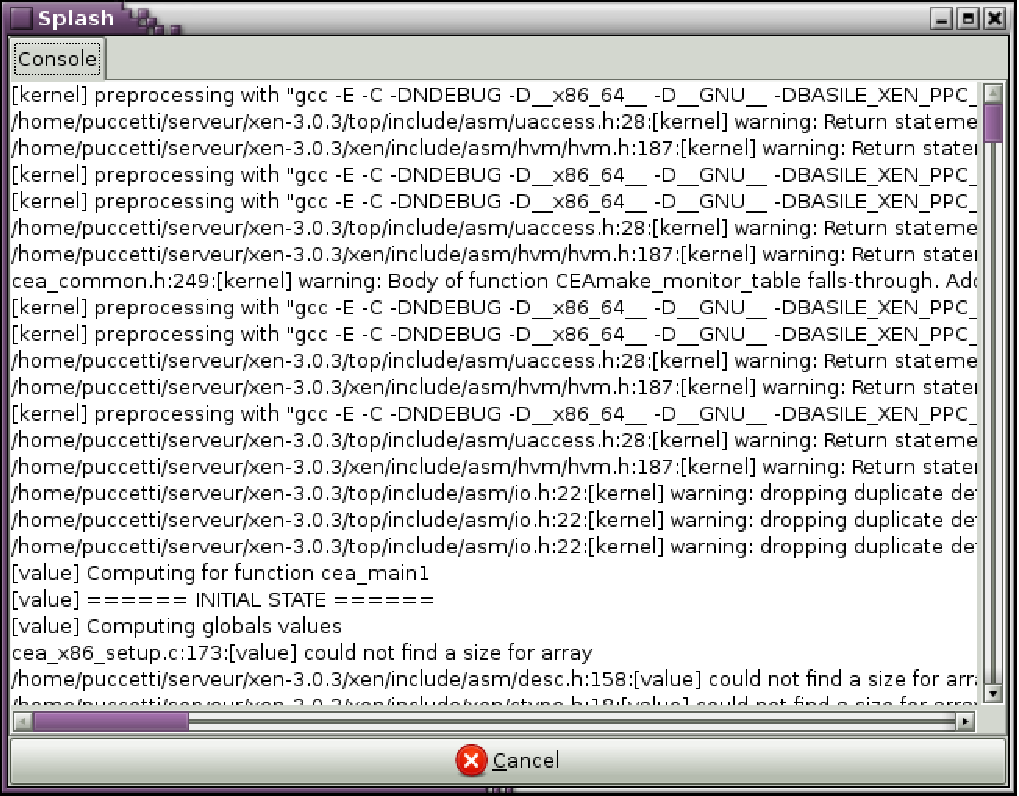
\includegraphics[width=\textwidth]{splash.pdf}
%% \end{center}
%% \caption{Splash Information View}
%% \label{sero}
%% \end{figure}

\section{Menu Bar}\label{sec:menubar}

The menu bar is organised as follows:
\begin{description}
\item [The file menu] proposes items for managing the current session.

\begin{description}
\item \texttt{Source files}: changes the analyzed files of
  the current project.
\item \texttt{Reparse}: reloads the source files of the current
  project from the disk, reparses them, and restarts the analyses that
  have been configured. % It is useful when testing \FramaC features on
  % source files that the user changes.
\item \texttt{Save session}: saves all the current projects into a file.
  If the user has not yet specified such a file, a dialog box is opened for
  selecting one.
\item \texttt{Save session as}: saves all current projects into a
  file chosen from a dialog box.
\item \texttt{Load Session}: opens a previously saved session.

  \begin{important}
  This fully resets the current session (see Section~\ref{sec:saveload}).
  \end{important}
\item \texttt{Exit Frama-C}: exits \FramaC without saving.
\end{description}

\item [The project menu] displays the existing projects, allowing you to set the
  current one. You can also perform miscellaneous operations over projects
  (creating from scratch, duplicating, renaming, removing, saving, \etc).

\item [The analyses menu] provides items for configuring and running plug-ins.

\begin{itemize}
\item \texttt{Analyses}: opens the dialog box shown in
  Figure~\ref{fig:launcher}, that allows setting \FramaC parameters and
  re-running analyses.
\begin{figure}[htbp!]
\begin{center}
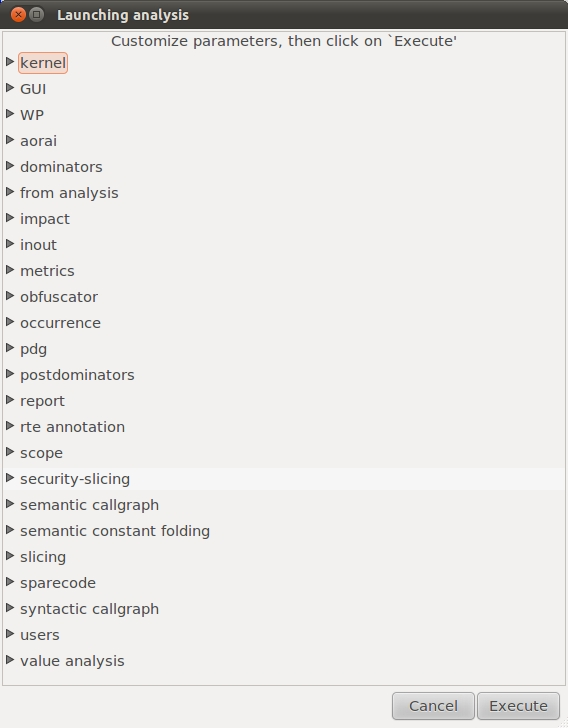
\includegraphics [scale=0.5] {analysis-window.jpg}
\end{center}
\caption{The Analysis Configuration Window}
\label{fig:launcher}
\end{figure}
\item \texttt{Load and run an OCaml module}: allows you to load a compiled \caml
  module as a plug-in (see Section~\ref{sec:use-plugins}).
\item Other items are plug-in specific.
\end{itemize}


\item [The debug menu] is only visible in debugging mode and provides access to
  tools for helping to debug \FramaC and their plug-ins.

\item [The help menu] provides help items.
\end{description}

\section{Tool Bar}\label{sec:toolbar}

The tool bar offers a more accessible access to some frequently used
functions of the menu bar.  Currently, the available buttons are, from left
to right:
\begin{itemize}
\item The \texttt{Exit} button, that exits \FramaC.

\item Four buttons \texttt{Source files}, \texttt{Reparse},
  \texttt{Load Session} and \texttt{Save session}, equivalent to the
  corresponding entries in the \texttt{File} menu.

\item Two navigation buttons, \texttt{Back} and \texttt{Forward}. They can
  be used to move within the history of the functions that have been viewed.

\item The \texttt{Analyses} button, equivalent to the one in the
  \texttt{Analyses} menu.

\item A \texttt{Stop} button, which halts the running
  analyses and restores \FramaC to its last known valid configuration.

\end{itemize}
